\chapter[Ruptures sismiques -- Glissement asismique]{Ruptures sismiques initiées par un glissement asismique}
\label{sec:chaparticle}
\vspace*{-0.5cm}


% Les failles sismiques sont composées de couches successives de roches, de cohésion et de granulométrie variables, mises en mouvement par cisaillement élastique. Elles arborent une physique riche et complexe, dont le comportement est difficilement prédictible, et les étudier est un enjeu scientifique majeur, tant pour leur compréhension que leur surveillance, et la prévention des séismes.

Les séismes, évènements rapides de rupture de l'interface, ne sont pas le seul moyen par lequel les failles relâchent l'énergie élastique qu'elles emmagasinent. Cette énergie peut également être libérée au travers d'évènements de glissement lent (Fig.\,\ref{fig:extract_review})\,\cite{peng_integrated_2010,burgmann_geophysics_2018}. Ces évènements lents ont tout d'abord été découverts dans les zones de subduction puis observés dans d'autres systèmes de failles, transformantes et en zones de décrochement (Fig.\,\ref{fig:typesdefailles}) avec l'amélioration des techniques de mesure\,\cite{harris_large_2017}. Ces séismes lents peuvent affecter de larges portions d'un système de failles, et relâcher des quantités d'énergie comparables à celles relâchées par les séismes rapides\,\cite{dragert_silent_2001}. Ils peuvent aussi être très localisés, et détectés indirectement par la déstabilisation de l'interface qui en résulte (phénomène nommé \textit{Episodic tremor and slip})\,\cite{chen_scaling_2009,shelly_non-volcanic_2007,tan_connecting_2020,rogers_episodic_2003}. Le rôle des zones de déplacement lent, dites \textit{asismiques} ou \textit{découplées}, sur la déstabilisation des zones en mouvement de stick-slip, dites \textit{sismiques} ou \textit{couplées}, reste pourtant méconnu\,\cite{radiguet_triggering_2016,dragert_silent_2001}.


\begin{figure}[h!]
\centering

\includegraphics[scale=1]{../Figures_chap_article/failles.pdf}
\caption[Types de failles]{Les trois grands types de failles. La faille normale (\textbf{a}) apparaît dans les systèmes en extension. La faille inverse (\textbf{b}) apparaît dans les systèmes en compression comme les zones de subduction. La faille transformante (\textbf{c}) apparaît dans les zones de coulissement entre des plaques tectoniques.}
\label{fig:typesdefailles}
\end{figure}


L'apparition de cette diversité de comportements, et la difficulté de leur étude, sont dues à la complexité des interfaces considérées. En effet celle-ci implique la prise en compte d'une multitude de paramètres, tels que la teneur en eau des roches, leur viscosité, leur nature, la géométrie des failles ou encore la présence d'une couche de gouge, une roche broyée non-cohésive, dans le système de failles. Les expériences en laboratoire telles que celles que nous avons menées nous donnent une opportunité unique d'analyser séparément l'influence de chacun de ces paramètres, en contrôlant les caractéristiques principales d'une interface frictionnelle, telles que sa composition, le chargement qui lui est appliqué, ou la présence d'hétérogénéités. Elles nous permettent également d'instrumenter densément le milieu, et de multiplier les expériences, et donc d'étudier l'influence de ces paramètres et de comprendre les mécanismes microscopiques responsables des phénomènes de grande échelle qui en émergent.

\pagebreak

Dans ce chapitre, nous étudions l'influence d'une hétérogénéité dans la composition de l'interface sur le comportement d'une faille sismique modèle. Cette interface prend dans notre étude la forme d'une interface frictionnelle solide-solide composée de deux plaques minces de polyméthacrylate de méthyle (PMMA) perturbée par l'inclusion d'un milieu granulaire dense sur une portion de sa longueur. La conclusion majeure des résultats présentés est qu'au sein d'une faille modèle, une hétérogénéité de composition à l'interface créé un patch en glissement lent entre les évènements sismiques. Ce patch s'étend au-delà de l'hétérogénéité et agit comme un précurseur de rupture, menant à la déstabilisation de l'interface frictionnelle par la propagation d'une rupture rapide. La longueur de ce patch est d'autant plus élevée que l'hétérogénéité est dense et chargée.

%Ce chapitre présente tout d'abord plus en détail le système d'interface en \textit{œil granulaire} étudié, et les observables que nous utiliserons pour décrire son comportement, puis présente nos observations expérimentales des modifications du cycle de stick-slip dues à l'inhomogénéité de composition, et présente enfin une discussion de ces résultats et les perspectives futures ouvertes par notre étude.


\begin{figure}[h!]
\centering
\includegraphics[scale=1]{../Figures_chap_article/extract_review.pdf}
\caption[Faille en glissement lent]{Structure et comportement d'une faille sismique subissant du glissement lent (extrait de\,\cite{burgmann_geophysics_2018}). \textbf{a.}\,Illustration schématique de la distribution du glissement sismique et asismique dans une portion de la faille transformante de San Andreas partiellement couplée. \textbf{b.}\,Distribution du glissement sismique et asismique sur une zone de subduction partiellement couplée.}
\label{fig:extract_review}
\end{figure}





\newpage

\minitoc


\newpage








\section{Système étudié -- définitions}

Cette section décrit l'interface en \textit{œil granulaire}, et le dispositif expérimental utilisé au cours des expériences analysées dans ce chapitre. Ce dispositif est détaillé dans le Chapitre\,\ref{sec:chapxp}. Nous introduisons également notre paramètre de contrôle, le \textit{contraste de chargement} $C_\sigma$ caractérisant la proportion du chargement normal porté par le milieu granulaire.




\subsection{Dispositif expérimental -- interface en œil granulaire}


\begin{figure}[htb]
\centering
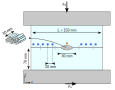
\includegraphics[scale=1]{../Figures_chap_article/schema.pdf}
\caption[Schéma de l'œil granulaire]{Schéma du dispositif expérimental utilisé. Les blocs de PMMA et l'œil mesurent respectivement \siprod{150x90x10}{\milli\meter} et \siprod{30x6x10}{\milli\meter}. Les grains, de diamètres $0.4$, $0.7$, $0.9$, et $1.3$\,mm (proportions en volume : 5, 10, 35 et 50\%) remplissent l'œil, et des grains de diamètre \SI{1.3}{\milli\meter} sont fixés aux parois de l'œil afin de le rugosifier. Les rosettes de jauges de déformation (carrés en bleu sombre et ocre) sont disposées à une distance de 2 à \SI{6}{\milli\meter} de l'interface. Huit motifs des faces des cylindres sont reproduits, par paires, le long de l'interface solide (cercles blancs).}
\label{fig:granuleyedetail}
\end{figure}



\subsubsection{Principe de l'expérience}

Le principe de l'expérience est de mettre en contact le long d'une interface frictionnelle deux solides élastiques, de leur appliquer un chargement cisaillant, et d'étudier le mouvement relatif des deux blocs. La particularité de notre dispositif est de pouvoir introduire un milieu granulaire au sein de cette interface solide-solide, sous la forme d'un patch localisé. Nous formons ainsi deux portions d'interface solide-solide, séparées par une portion d'interface granulaire. L'introduction de cette inclusion granulaire induit une modification de la réponse en cisaillement de l'interface. Dans cette étude, nous mettons en évidence les mécanismes locaux responsables de cette modification.

%Les objectifs de cette inclusion sont l'observation de la modification de la réponse en cisaillement de l'interface en fonction de la densité du milieu granulaire, et la compréhension des mécanismes locaux responsables de celle-ci.

\newpage

\subsubsection{Dispositif et mesures}

Nous étudions une interface frictionnelle quasi-1D formée par les surfaces solides macroscopiquement lisses de deux blocs de PMMA, tenus par des mors métalliques. Un trou elliptique est percé au centre de l'interface. Le trou, ou \textit{œil}, est rempli de grains cylindriques en nylon, de diamètres compris entre $0.4$ et \SI{1.3}{\milli\meter}. Le nombre de grains est variable d'une expérience à l'autre. Des cylindres sont collés dans des rainures usinées dans les surfaces de l'œil afin de
s'assurer que le cisaillement est transmis aux grains libres présents dans le volume de l'œil.
%les solidariser au milieu granulaire.
Cette interface est alors pressée par une force $F_N$, puis cisaillée par le bas du bloc inférieur, à une vitesse constante de \SI{20}{\micro\meter\per\second}, ce qui exerce une force cisaillante $F_S$ sur l'interface (Fig.\,\ref{fig:granuleyedetail}). Les deux forces sont mesurées à \SI{315}{\hertz}. Dans la plupart des expériences que nous avons menées, nous nous sommes placés à $F_N\simeq\SI{3000}{\newton}$ et avons fait varier la densité du milieu granulaire. Seules certaines expériences de référence, sans grains, ou avec des blocs solides lisses (sans œil), ont été effectuées à force normale variable.



Le bloc inférieur est instrumenté de 10 rosettes de 3 jauges de déformation installées le long de l'interface, permettant de mesurer le tenseur des déformations $\varepsilon$.
%Nous mesurons ce tenseur en 10 points de mesure choisis en raison des limitations techniques de notre matériel d'amplification, 
Les mesures présentées dans ce chapitre ont été effectuées avec le jeu de cartes DIP (Sec.\,\ref{sec:anderson}). L'acquisition est réalisée continûment à \SI{315}{\hertz}, ainsi que par salves de \SI{10}{\milli\second} à \SI{4}{\mega\hertz} lors des évènements de glissement rapide (Sec.\,\ref{sec:electronique}). Grâce à l'hypothèse de planéité des contraintes (\textit{plane stress}) permise par la géométrie 2D du système mécanique, les tenseurs des déformations et des contraintes sont définis par seulement trois composantes, mesurées par les rosettes.


En parallèle de l'acquisition électronique, nous effectuons un suivi optique de l'interface. Les faces des cylindres sont peintes d'un motif spécifique, et imagées à l'aide d'une caméra à 100 images par secondes. Ce motif spécifique est reproduit au-dessus des parties solides de l'interface afin d'en permettre le suivi. Leur position est déterminée à l'aide d'un algorithme de suivi de particules (PTV), à une précision de l'ordre de \SI{5}{\micro\meter} (Sec.\,\ref{sec:optique}).



\subsection{Remplissage de l'œil granulaire -- contraste de chargement}

Nous avons effectué deux types d'expériences :

\begin{itemize}
\bitem Expériences \textit{à vide} : l'œil est laissé vide de grains, l'interface consiste alors en deux portions d'interface solide-solide séparées par un trou.
\bitem Expériences \textit{granulaires} : l'œil est rempli par suffisamment de cylindres (soit une centaine) pour assurer que les blocs solides exercent une pression sur le milieu granulaire.
\end{itemize}

Dans le cas des expériences granulaires, il est possible de faire varier le nombre de cylindres emprisonnés dans l'œil, et donc la densité du milieu granulaire. Cette densité est de l'ordre de 60\%, et du fait de la compacité du milieu, elle varie peu avec le nombre de grains. Ainsi l'ajout de quelques cylindres suffit à passer d'un état proche de la situation à vide à un état où le milieu granulaire porte la majeure partie de la charge appliquée à l'interface.
Dans ces expériences nous sommes vigilants à ce que les interfaces solide-solide ne soient jamais entièrement déchargées.
%, sans jamais décharger entièrement les portions solide-solide.
Afin de caractériser ces variations nous définissons le \textit{contraste de chargement} $C_\sigma$ comme la différence de chargement normal entre les portions solides de l'interface et l'œil granulaire, normalisée par le chargement total moyen, c'est à dire

\begin{equation}
C_\sigma=\dfrac{\sigma_{yy}^{gran}-\left\langle \sigma_{yy}^{solid} \right\rangle}{\left\langle\sigma_{yy}\right\rangle}
\end{equation}


Ce paramètre varie continûment. Du fait de la normalisation par le chargement moyen, il permet de s'affranchir des variations de $F_N$ autour de sa valeur de consigne de \SI{3000}{\newton}. Pour les expériences à vide $C_\sigma\simeq-1$, tandis que pour les expériences granulaires que nous avons menées, $-1<C_\sigma<2.5$. La limite haute du contraste de chargement est le déchargement des sections solide-solide, menant à un glissement stable de l'interface.


\begin{figure}[h!]
\centering
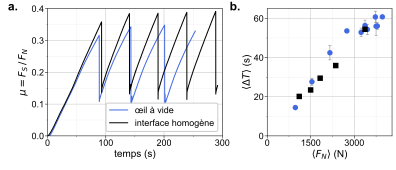
\includegraphics[scale=1]{../Figures_chap_article/ss_vs_eh.pdf}
\caption[Comparaison interface homogène -- œil à vide]{\textbf{a.}\,Cycle de stick-slip pour une expérience solide-solide (en noir) et une expérience à vide (en bleu sombre). Les deux expériences sont effectuées à force normale constante $F_N\sim\SI{3000}{\newton}$. \textbf{b.}\,Période moyenne du stick-slip en fonction de la force normale appliquée sur le système, pour plusieurs expériences solide-solide (carrés noirs) et à vide (cercles bleus).}
\label{fig:comparsolidempty}
\end{figure}



\section{Modification de la fréquence de stick-slip}
\label{sec:modiffreq}

Lors d'une expérience, les blocs sont pressés avec une force $F_N \sim \SI{3000}{\newton}$, et cisaillés sur une distance d'environ \SI{5}{\milli\meter} à une vitesse de \SI{20}{\micro\meter\per\second}. Lors de ce déplacement, le système frictionnel subit, quel que soit la configuration ou le contraste de chargement, un mouvement de stick-slip. Les propriétés de ce mouvement, en particulier sa périodicité, sont cependant affectées par les valeurs de $F_N$ et $C_\sigma$. Dans cette section, nous montrons que la présence de l'œil granulaire entraîne une diminution de la période de stick-slip. Cette réduction est d'autant plus prononcée que le contraste de chargement augmente.


\subsection{Interface solide-solide homogène -- Interface à trou}


Lors d'une expérience de cisaillement avec des blocs homogènes macroscopiquement plats, c'est à dire sans œil, le mouvement relatif des surfaces formant l'interface est un mouvement de stick-slip. Afin de caractériser l'influence de l'œil granulaire sur le comportement de l'interface, nous nous sommes d'abord intéressés à l'effet du changement de géométrie sur celui-ci. En effet la présence de l'œil, même vide, pourrait suffire à le perturber. Pour chaque expérience, nous mesurons les temps $\{T_i\}_{i\in\mathbb{N}}$ auxquels des évènements de glissement rapide ont lieu, et définissons la période moyenne du mouvement $\left\langle\Delta T\right\rangle = \left\langle T_{i+1}-T_i\right\rangle_{i\in\mathbb{N}}$.

Nous nous attendons, dans de telles conditions expérimentales, à ce que la période du stick-slip soit indépendante de la géométrie des blocs, et soit proportionnelle à la force normale appliquée sur l'interface (Éq.\,\ref{eq:freqss}). Nos mesures montrent bien cette indépendance (Fig.\,\ref{fig:comparsolidempty}), puisqu'à force normale variable, la variation de $\mean{\Delta T}$ entre les expériences solide-solide et avec l'œil à vide est inférieure à 10\%. Cet écart peut s'expliquer par les variations
attendues du coefficient de frottement statique pour un système donné entre deux séries d'expériences\,\cite{ben-david_static_2011}.
Les multiples mesures prises pour l'œil à vide à $F_N=\SI{3000}{\newton}$ au cours de plusieurs séries d'expériences différentes présentent en effet une variation similaire. Ainsi la présence de l'œil à l'interface en tant que défaut purement géométrique n'a pas d'influence sur son comportement, en particulier sur le cycle de stick-slip.

\newpage

\subsection{Expériences granulaires}

\begin{figure}[htb]
\centering
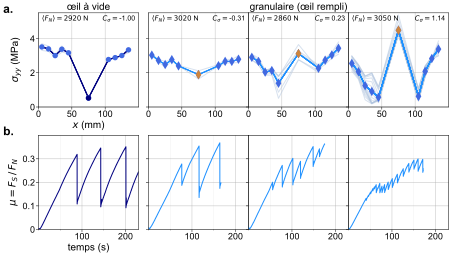
\includegraphics[scale=1]{../Figures_chap_article/figure_1_c_d.pdf}
\caption[Contraste de chargement $C_\sigma$]{Comportement macroscopique de l'interface frictionnelle. \textbf{a.}\,Profil de chargement normal d'une expérience à vide (gauche) et de trois expériences granulaires (droite). Le profil moyen (en couleur) est déterminé comme la moyenne des profils de chargement juste avant chaque évènement de glissement rapide (en gris). Ce profil est utilisé pour déterminer $C_\sigma$. Les cercles indiquent une expérience à vide, les diamants une expérience granulaire. Les symboles en bleu clair indiquent les mesures prises au-dessus des portions solides de l'interface. Les cercles en bleu sombre indiquent une mesure prise au-dessus de l'œil à vide, et les diamants ocres au-dessus de l'œil granulaire plein. \textbf{b.}\,Évolution temporelle de $\mu=F_S/F_N$ correspondant à chaque expérience présentée, ligne sombre pour une expérience à vide, et claire pour les expériences granulaires.}
\label{fig:loadingcontrast}
\end{figure}



Afin d'étudier l'influence du milieu granulaire, nous avons rempli l'œil d'une quantité variable de grains. Nous nous plaçons à force normale fixée, $F_N=\SI{3000}{\newton}$, cette force variant peu au cours d'une expérience. Le paramètre que nous faisons varier est le nombre de grains dans l'œil, c'est à dire la densité du milieu granulaire. Nous caractérisons cette densité par le contraste de chargement $C_\sigma$. Lorsque nous effectuons les mêmes expériences que celles décrites précédemment, mais avec l'œil granulaire rempli, nous observons toujours un mouvement de stick-slip, seulement sa période est diminuée relativement à celle des expériences à vide (Fig.\,\ref{fig:loadingcontrast}). Cette variation de la période peut aller d'une simple perturbation lorsque $C_\sigma\sim-1$ à une réduction par un facteur 10 lorsque $C_\sigma\sim 2$ (Fig.\,\ref{fig:freqlc}). Nous observons également que les chutes de forces, plus faibles en raison de la diminution de la période, sont d'une amplitude moins régulière.



Dans les expériences solide-solide homogène et à vide, la période du stick-slip est proportionnelle à la force normale appliquée à l'interface, et donc à la contrainte normale qu'elle porte. Par ailleurs dans les expériences granulaires nous observons qu'une augmentation de $C_\sigma$ entraîne une diminution de la contrainte normale portée par les portions solide-solide de l'interface $\sigma_{yy}^{solid}$ (Fig.\,\ref{fig:loadingcontrast}). Il pourrait donc être possible que la variation que nous observons dans les expériences granulaires soit due à ce déchargement, et que l'œil granulaire n'agisse que par la réduction du chargement porté par les portions solide-solide de l'interface. Afin de tester cette hypothèse, nous mesurons les variations de la période du mouvement de stick-slip $\mean{\Delta T}$ en fonction de la moyenne de la contrainte normale portée par les portions solide-solide de l'interface $\mean{\sigma_{yy}^{solid}}$ dans des expériences granulaires à différents $C_\sigma$ sous une force normale $F_N\simeq \SI{3000}{\newton}$ (Fig.\,\ref{fig:frequencyfn}, diamants). Une comparaison avec des expériences à vide et solide-solide homogène pour différentes forces normales révèle que la variation de période induite par le milieu granulaire est supérieure à celle qui serait induite par un simple déchargement des sections solide-solide de l'interface.

Ces deux observations démontrent que l'hétérogénéité de composition que constitue l'œil granulaire et l'augmentation de $C_\sigma$ sont responsables de la réduction de $\mean{\Delta T}$, et de la déstabilisation de l'interface. Nous allons à présent déterminer les mécanismes responsables de cette diminution.


\begin{figure}[h!]
\centering
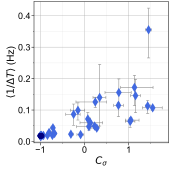
\includegraphics[scale=1]{../Figures_chap_article/lc_vs_freq.pdf}
\caption[Fréquence de stick-slip en fonction de $C_\sigma$]{Variation de la fréquence de stick-slip en fonction de $C_\sigma$. Les expériences à vide sont représentées par des cercles en bleu sombre, et les expériences granulaires par des diamants en bleu clair.}
\label{fig:freqlc}
\end{figure}


\begin{figure}[h!]
\centering
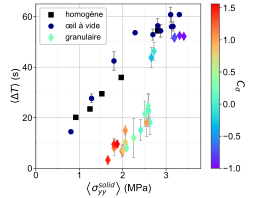
\includegraphics[scale=1]{../Figures_chap_article/figure_1_b.pdf}
\caption[Fréquence du stick-slip en fonction de la contrainte normale]{Période moyenne du stick-slip en fonction du chargement moyen des sections solide-solide de l'interface. Les expériences de référence avec interface solide-solide homogène, à force normale variable, sont représentées par des carrés noirs, les expériences avec œil à vide, à force normale variable, par des cercles, et les expériences granulaires à force normale $F_N\sim\SI{3000}{\newton}$, à contraste de chargement $C_\sigma$ variable, par des diamants. La couleur des diamants indique la valeur de $C_\sigma$.}
\label{fig:frequencyfn}
\end{figure}




\section{Observation d'un glissement lent}


La modification de la période du stick-slip est la manifestation macroscopique du comportement de l'interface, mais quel est le mécanisme local qui en est à l'origine ? Nous disposons pour répondre à cette question de mesures locales de déplacements et de déformations.

%Afin de déterminer le mécanisme à l'œuvre dans la déstabilisation de l'interface, nous suivons optiquement les déplacements des faces des cylindres solidaires des blocs, ainsi que des faces de cylindres reproduites de part et d'autre des portions solide-solide de l'interface.

%
%\subsection{Attentes quand à la mesure des déplacements}
%\begin{figure}
%\centering
%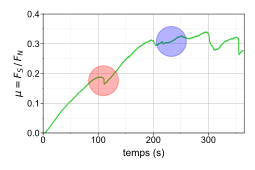
\includegraphics[scale=1]{../Figures_chap_article/fully_gran.pdf}
%\caption{Évolution de $\mu=F_S/F_N$ pour une interface entièrement granulaire, sous un chargement normal de $F_N=\SI{3000}{\newton}$. Des évènements de glissement rapide sont observés (cercles rouges) ainsi que des phases de glissement lent (cercles bleus).}
%\label{fig:fullygranss}
%\end{figure}
%
%
%Notre objectif initial regardant cette mesure optique était d'effectuer un suivi à haute vitesse (de l'ordre de \num{500000} images par seconde) de chaque grain, au sein d'une interface entièrement granulaire (décrite en Section\,\ref{sec:geometriedesblocs}), et au cours d'évènements de glissement rapide. Nous souhaitions observer la propagation d'un front de rupture au sein du milieu granulaire, et avons développé à cet effet un algorithme de suivi nous permettant une résolution de l'ordre de \SI{5}{\micro\meter}. Nous avons alors observé que le système entièrement granulaire ne subissait pas un cycle de stick-slip, mais un mouvement moins défini, comportant des évènements de glissement rapide, des phases de chargement sans mouvement, et des phases de glissement lent (Fig.\,\ref{fig:fullygranss}). Ainsi nous avons émis l'hypothèse que l'œil granulaire puisse être en glissement lent entre les évènements de glissement rapide, et avons cherché à mesurer ce glissement.


\subsection{Mesure du glissement interfacial}

\subsubsection{Définition des grandeurs observées}

Afin d'étudier les déplacements à l'interface nous définissons plusieurs grandeurs à partir des mesures brutes des positions des cylindres. Une définition détaillée de ces grandeurs est disponible dans le Chapitre\,\ref{sec:chapxp}, Section\,\ref{sec:obsoptique}.

\begin{itemize}
\bitem Chaque évènement de glissement rapide est repéré par un temps $t_k$. Les bornes de l'évènement sont définies comme $\left[t_k-\tau^-\,,\,t_k+\tau^+\right]$, où $\tau^-=\SI{50}{\milli\second}$, et $\SI{150}{\milli\second}\leq\tau^+\leq\SI{500}{\milli\second}$.
\bitem Le \textit{déplacement interfacial}, noté $\delta_{tot}(t)$, est défini comme la différence de position moyenne entre les cylindres du bloc supérieur et ceux du bloc inférieur.
\bitem Le \textit{glissement inter-évènement}, noté $\delta_{IE}(t)$, est défini comme le cumul de la distance glissée entre les évènements de glissement rapide. Il peut s'exprimer comme
\begin{equation}
\delta_{IE}(t)=\delta_{tot}(t)-\sum_{t_k\leq t}\Big(\:\delta_{tot}(t_k^+)-\delta_{tot}(t_k^-)\:\Big)
\end{equation}
Il est représenté comme la suite de ses valeurs aux temps ${\{t_k+\tau^+\}_{k\in\mathbb{N}}}$.
\bitem Le \textit{glissement inter-évènement normalisé} $S(t)$, est la proportion de glissement se faisant entre les évènements de glissement rapide. Tout comme $\delta_{IE}$, il est représenté dans notre étude comme la suite de ses valeurs aux temps $\{t_k+\tau^+\}_{k\in\mathbb{N}}$. Il s'exprime comme
\begin{equation}
S(t)=\delta_{IE}(t)/\delta_{tot}(t)
\end{equation}
\end{itemize}



Ces trois dernières quantités peuvent dépendre de la position à laquelle elles sont mesurées. Afin d'en rendre compte, nous les définissons pour des portions d'interfaces (Sec.\,\ref{sec:classement}). Nous noterons alors $\delta_{tot}^{\{l\}}$ le déplacement interfacial d'une portion, où $\{l\}$ est \textit{eye} pour l'œil granulaire et \textit{solid} pour les portions solide-solide de l'interface.
%Elles peuvent aussi être définies pour une position précise repérée par deux cylindres de par et d'autre de l'interface, auquel cas la position est indiquée comme paramètre.



Il est possible de relier $S(t)$ au couplage $\phi$ de l'interface, qui quantifie le fait qu'une interface soit bloquée ou en glissement permanent. Le couplage est défini par le rapport de la vitesse de glissement $v_{slip}$ d'une faille et de sa vitesse de chargement $v_{load}$ comme $\phi=1-{v_{slip}}/{v_{load}}$


\subsubsection{Exemple d'une expérience simulée}



Afin d'illustrer les définitions que nous venons d'effectuer, nous les explicitons dans le cas d'un mouvement simulé (détail en Sec.\,\ref{sec:obsoptique}). Afin de simuler un mouvement de stick-slip comportant du déplacement lent entre les évènements de slip, nous contrôlons la position du bloc inférieur non-chargé, au moyen de la platine motorisée, pilotée par un script (Fig.\ref{fig:deltaart}a). Les cylindres solidaires du bloc sont suivis par imagerie. Les instructions données sont des cycles de 5 secondes sans mouvement, 5 secondes de déplacement uniforme à \SI{20}{\micro\meter\per\second} (glissement lent), et un saut brusque de \SI{100}{\micro\meter} (évènement de slip).

Dans le cas de cette expérience simulée, les évènements $\{t_k\}$ correspondent aux sauts brusques, $\delta_{IE}(t)$ correspond au déplacement cumulé durant les phases de \SI{5}{\second} de déplacement uniforme à \SI{20}{\micro\meter\per\second}, et augmente donc de \SI{100}{\micro\meter} entre chaque évènement (Fig.\,\ref{fig:deltaart}b). La valeur attendue de $S(t)$ est donc de 50\%. Les valeurs mesurées pour $\delta_{IE}(t)$ et $s(t)$ sont 1 à 2\% plus faibles que les valeurs attendues en raison de la largeur $\tau^-+\tau^+$ prise autour des évènements (Fig.\,\ref{fig:deltaart}c). Cette mesure synthétique montre que nos méthodes d'analyse fournissent les résultats attendus, sinon que les valeurs obtenues sont très légèrement sous-estimées.




\begin{figure}[p]
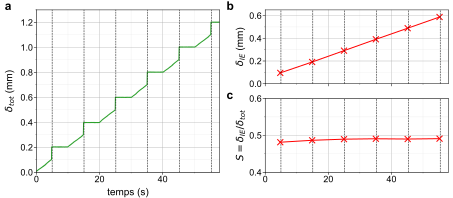
\includegraphics[scale=1]{../Figures_chap_exp/figure_S2_delta_only.pdf}
\caption[Exemple de mouvement scripté]{Déplacement d'un seul des blocs commandé par un script. \textbf{a.}\,Mesure du déplacement interfacial $\delta_{tot}$. Les évènements détectés sont marqués par les lignes en pointillés noirs. \textbf{b.}\,Évolution du glissement inter-évènement $\delta_{IE}$. \textbf{c.}\,Évolution du glissement inter-évènement normalisé $S$.}
\label{fig:deltaart}
\end{figure}

\begin{figure}[p]
\centering
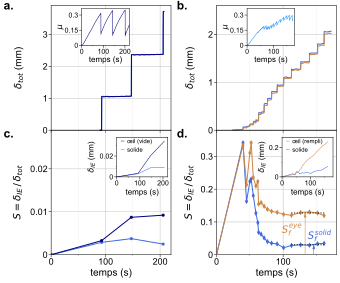
\includegraphics[scale=1]{../Figures_chap_article/figure_2.pdf}
\caption[Mesures du glissement interfacial]{Mesures du glissement interfacial. \textbf{a-b.}\,Évolution temporelle du glissement interfacial total $\delta_{tot}^{\{l\}}$ pour les sections solide-solide (bleu clair), l'œil à vide (\textbf{a},\,bleu sombre) et plein (\textbf{b}, ocre). Les deux expériences présentées sont celles de la Figure\,\ref{fig:loadingcontrast} (à vide, et granulaire à $C_\sigma$ le plus élevé). En encart les courbes de $\mu=F_S/F_N$ associées. \textbf{c-d.}\,Évolution temporelle du glissement inter-évènement normalisé $S^{\{l\}}$. En encart le glissement inter-évènement (non-normalisé) $\delta_{IE}^{solid}$ et $\delta_{IE}^{eye}$.}
\label{fig:papier2}
\end{figure}


\subsection{Glissement de l'œil granulaire}

\subsubsection{Évolution temporelle du glissement}


Nous réalisons les mesures de déplacement le long des portions solide-solide et le long de l'œil dans des expériences à vide et granulaires (Fig.\,\ref{fig:papier2}a-b) et nous déterminons $S(t)$ le glissement inter-évènement normalisé (Fig.\,\ref{fig:papier2}c-d). Dans le cas de l'expérience à vide présentée, $S(t)$ converge vers une valeur de l'ordre de 1\%, indiquant que l'interface est entièrement bloquée. Pour l'ensemble des expériences à vide le glissement inter-évènement normalisé est faible, $S^{\{l\}}(t)<0.02$, c'est à dire que moins de 2\% du déplacement total s'effectue entre les évènements de glissement rapide, indiquant que toute l'interface est verrouillée. Dans le cas de l'expérience granulaire présentée, l'œil granulaire subit un glissement inter-évènement normalisé de l'ordre de $S^{eye}\sim 0.13$ une fois convergé, tandis que les portions solide-solide restent presque verrouillées, avec $S^{solid}\sim 0.04\ll S^{eye}$. Cette tendance est généralisée dans toutes les expériences granulaires, et s'intensifie avec l'augmentation de $C_\sigma$.

Dans le cas des expériences à œil granulaire, $S$ varie initialement beaucoup (Fig.\,\ref{fig:papier2}d), car il est défini comme une division de deux quantités qui sont initialement faibles et subissent une grande influence du bruit de mesure. Cependant à temps long, $\delta_{IE}$ et $\delta_{tot}$ étant des valeurs cumulées, $S$ converge. Le critère que nous utilisons en pratique est de retenir pour valeur de $S$ la moyenne des 5 derniers points de mesure $S_f$, et pour barre d'erreur l'écart type de celles-ci.




\subsubsection[Évolution du glissement en fonction de $C_\sigma$]{Évolution du glissement en fonction du contraste de chargement}

\begin{figure}[htb]
\centering
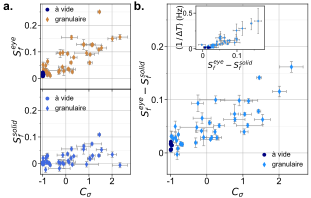
\includegraphics[scale=1]{../Figures_chap_article/figure_3.pdf}
\caption[Mesures du glissement lent]{Mesures du glissement lent. \textbf{a.}\,Valeurs convergées du glissement inter-évènement normalisé en fonction de $C_\sigma$. En haut, $S_f^{eye}$ pour les expériences à vide et granulaires. En bas, $S_f^{solid}$. \textbf{b.}\,Valeurs convergées du glissement inter-évènement normalisé relatif $S_f^{eye}-S_f^{solid}$ en fonction du contraste de chargement. En encart, fréquence du stick-slip en fonction de $S_f^{eye}-S_f^{solid}$.}
\label{fig:papier3}
\end{figure}




À partir des mesures de $S(t)$, nous mesurons $S_f^{eye}$ et $S_f^{solid}$ pour l'ensemble de nos expériences. Ces deux quantités sont des fonctions croissantes de $C_\sigma$ (Fig.\,\ref{fig:papier3}a). Ainsi plus l'œil granulaire est chargé, plus l'interface glisse durant les périodes inter-évènement au niveau de l'œil, mais également au niveau des portions solide-solide. Cependant $S_f^{solid}$ reste systématiquement plus faible que $S_f^{eye}$. Les portions solide-solide ne glissent pas ou peu entre les évènements, et la partie granulaire effectue jusqu'à 20\% de son déplacement durant ces phases. Afin d'isoler la proportion de glissement spécifique à l'œil granulaire, nous mesurons la différence de glissement entre l'œil et les portions solide-solide $S_f^{eye}-S_f^{solid}$. Cette différence de glissement est également croissante avec $C_\sigma$ (Fig.\,\ref{fig:papier3}b). Par ailleurs, cette quantité est positivement corrélée à la fréquence du mouvement de stick-slip $\mean{1/\Delta T}$ (Fig.\,\ref{fig:papier3}b, encart).


Ainsi nous avons mis en évidence l'existence d'un patch glissant lentement entre les évènements de glissement rapide, situé au niveau de l'œil granulaire. L'écart de glissement inter-évènement entre ce patch et les portions solide-solide de l'interface, $S_f^{eye}-S_f^{solid}$, augmente avec $C_\sigma$. Une augmentation de la proportion de glissement lent entre les évènements mène à une déstabilisation précoce de l'interface frictionnelle.


\subsection{Évolution spatiale du glissement}

\begin{figure}[htb]
\centering
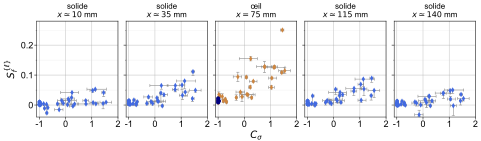
\includegraphics[scale=1]{../Figures_chap_article/creep_5_paires.pdf}
\caption[Glissement inter-évènement le long de l'interface]{Glissement inter-évènement normalisé convergé $S_f$ en fonction de $C_\sigma$ en 5 points de mesure, tout le long de l'interface.}
\label{fig:creep_5_paires}
\end{figure}



La mesure du glissement inter-évènement que nous avons effectuée rend compte du déplacement moyen des cylindres pour les sections solide-solide et pour l'œil granulaire. L'augmentation de $S_f^{solid}$ avec $C_\sigma$ peut donc s'expliquer comme l'augmentation d'un glissement homogène tout le long des portions solide-solide, ou comme un élargissement d'une zone glissante localisée, centrée sur l'œil granulaire.

Pour déterminer le mécanisme à l'œuvre dans cette augmentation, nous avons mesuré le glissement inter-évènement en différents points de l'interface, au niveau de chaque paire de faces de cylindre dessinées dans les parties solide-solide, et au-dessus du milieu granulaire (Fig.\,\ref{fig:creep_5_paires}). Cette mesure montre que plus le point de mesure est proche de l'œil granulaire, plus l'augmentation de $S_f$ avec $C_\sigma$ est marquée. Elle tend même à montrer, pour les deux points solide-solide les plus proches de l'œil, un seuil en $C_\sigma\simeq 0$ à partir duquel $S_f$ augmente. Cette mesure montre l'existence d'un patch glissant étendu, ne se limitant pas à l'œil granulaire, mais s'étendant à une partie de l'interface solide-solide lorsque $C_\sigma$ augmente. La mesure de sa longueur est effectuée dans la suite de notre étude (Sec.\,\ref{sec:longueurpatch}).


Ainsi nous avons montré dans cette section que l'inclusion d'une hétérogénéité à l'interface sous la forme d'un œil granulaire induit l'apparition d'un patch glissant. Ce patch glisse d'autant plus que le milieu granulaire est dense, et l'œil chargé. Le glissement du patch est corrélé à l'augmentation de fréquence du mouvement de stick-slip, et il est raisonnable de penser qu'il en est à l'origine. De plus l'augmentation de $S_f^{solid}$ avec $C_\sigma$ indique que le patch glissant n'est pas limité à la seule extension de l'œil granulaire. Si cette extension spatiale évolue en fonction de $C_\sigma$, sa mesure nécessite de pouvoir distinguer une section glissante d'une section bloquée de l'interface.



La confirmation de la présence de ce patch glissant nous est donnée par la mesure des déformations le long de l'interface, en particulier la détermination du point de nucléation des évènements de glissement rapide et l'évolution lente des contraintes cisaillantes au cours des phases inter-évènement. Ces deux observations et les conclusions que nous en tirons sont décrites dans les deux sections suivantes.




\section{Effet du glissement lent sur la nucléation des ruptures}

\subsection{Contexte}
\label{sec:nuccontexte}

Les évènements de glissement rapide subits par une interface frictionnelle sont tous initiés par la propagation d'une rupture le long de l'interface. Ce phénomène a été observé dans de nombreux matériaux analogues\,\cite{nielsen_experimental_2010,
rubinstein_detachment_2004,
svetlizky_brittle_2019,
xia_laboratory_2004}, des roches\,\cite{mclaskey_slow_2017,
passelegue_sub-rayleigh_2013,xu_strain_2018} et en présence d'une couche de gouge\,\cite{buijze_effects_2021,
ma_period_2001}.
Ce sont des ruptures décrites par la mécanique de la fracture linéaire élastique (Sec.\,\ref{sec:LEFM})\,\cite{svetlizky_brittle_2019}.

La rupture associée à un évènement rapide démarre en un point de l'interface nommé \textit{point de nucléation}, puis se propage à partir de ce point à toute l'interface à une vitesse pouvant atteindre la vitesse du son dans le matériau des blocs, affaiblissant à son passage les microcontacts entre les deux blocs. Les microcontacts affaiblis se mettent alors en glissement, et la contrainte cisaillante $\sigma_{xy}$ qu'ils supportent localement décroît d'une valeur initiale $\sigma_{xy}^0$ à une \textit{contrainte résiduelle} $\sigma_r$. Une fois l'interface entièrement affaiblie, elle se met à glisser dans son ensemble au cours d'un mouvement inertiel, entraînant une deuxième chute de contrainte de plus grande amplitude\,\cite{passelegue_frictional_2016}. Dans le patch en glissement lent, les contacts sont déjà affaiblis, et supportent déjà une contrainte cisaillante de $\sigma_r$, ils ne peuvent donc plus casser. La rupture ne peut y nucléer ni s'y propager. Les contraintes supportées par le patch diminuent tout de même au cours d'un évènement en raison du déplacement inertiel de l'interface.


Ainsi une augmentation de la fréquence des évènements rapides, comme celle observée dans nos expériences, correspond à une augmentation de la fréquence à laquelle une rupture nuclée et se propage. De plus la nucléation ne peut avoir lieu que dans une portion bloquée de l'interface. Il est donc possible, à l'aide de la détection des points de nucléation, d'effectuer une première évaluation de la longueur du patch glissant. Nous montrons dans cette section que le patch glissant s'élargit lorsque le contraste de chargement augmente et agit comme un déclencheur pour la nucléation d'une rupture, entraînant une déstabilisation précoce de l'interface.



\subsection{Élargissement du patch glissant}

\subsubsection{Cas de référence à vide}

\begin{figure}[htb]
\centering
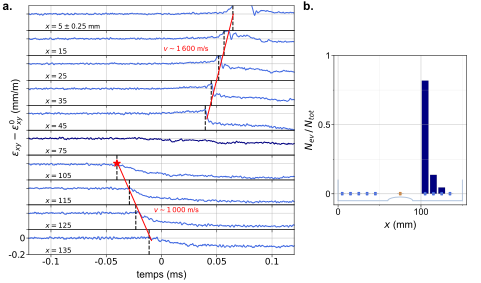
\includegraphics[scale=1]{../Figures_chap_article/hist_eh.pdf}
\caption[Nucléation et propagation -- expérience à vide]{\textbf{a.}\,Propagation d'une rupture dans une expérience à vide. Le point de nucléation est signalé par une étoile rouge. Les traits rouges indiquent une estimation de la vitesse de propagation de la rupture. \textbf{b.}\,Histogramme représentant la distribution des positions du point de nucléation pour les expériences à vide. Chaque barre correspond au nombre de ruptures s'étant initiées au niveau de la jauge associée $N_{ev}$, normalisé par le nombre total de ruptures $N_{tot}$.}
\label{fig:propagss}
\end{figure}


Le cas que nous utilisons comme référence est celui des expériences à vide, dont nous avons montré qu'elle est équivalente à une interface solide-solide homogène. La mesure de $\varepsilon_{xy}$ au cours d'un évènement de glissement (Fig.\,\ref{fig:propagss}a) montre que pour chaque point de mesure $x_i$ le cisaillement local quitte sa valeur initiale $\varepsilon_{xy}^0(x_i)$ à un instant $t_i$ au passage d'une rupture (lignes pointillées).
%Son évolution au cours de la centaine de microsecondes suivant $t_i$ est dictée par les fonctions angulaires de la mécanique de la fracture linéaire élastique\,\cite{freund_dynamic_1990,svetlizky_brittle_2019}, et 
Au cours de la centaine de microsecondes suivant $t_i$ elle décroît vers la valeur correspondant à la contrainte résiduelle locale\,\cite{freund_dynamic_1990,svetlizky_brittle_2019}.
% Cette évolution est contrôlée par la mécanique de la fracture linéaire élastique (Sec.\,\ref{sec:LEFM}), cependant en raison des différents [...] nos signaux ne correspondent pas à ses prédictions...
La chute de déformations (\textit{strain drop}) $\Delta\varepsilon_{xy}(x,t)$ est définie comme

\begin{equation}
\Delta\varepsilon_{xy}(x,t)=\varepsilon_{xy}(x,t)-\varepsilon_{xy}^0(x)
\end{equation}

L'instant $t_i$ auquel la chute de déformation a lieu diffère d'un point de mesure à l'autre, ce qui permet de suivre la propagation de la rupture. La position de la première jauge à quitter sa valeur initiale $\varepsilon_{xy}^0(x_{nuc})$ correspond au point de nucléation $x_{nuc}$. Les temps de passage de la rupture au niveau des autres points de mesure permettent de déterminer sa vitesse de propagation. Dans le cas de l'expérience à vide présentée dans la Figure\,\ref{fig:propagss}a, le point de nucléation de la rupture est mesuré à la position $x_{nuc}=\SI{105}{\milli\meter}$ (étoile rouge), et sa vitesse de propagation $v$ est différente de part et d'autre du point de nucléation, avec $v\sim\SI{1600}{\meter\per\second}$ vers les $x$ négatifs et $v\sim\SI{1000}{\meter\per\second}$ vers les $x$ positifs (lignes rouges). Dans nos expériences nous avons observé des ruptures \textit{sub-Rayleigh}, c'est à dire se propageant à une vitesse $v<c_r$ avec $c_r\simeq\SI{1250}{\meter\per\second}$ la vitesse des ondes de Rayleigh dans le PMMA, et des ruptures \textit{supershear} ($v$>$c_s\simeq\SI{1350}{\meter\per\second}$ la vitesse des ondes de cisaillement dans le matériau\,\cite{christman_dynamic_1972}). La gamme de vitesses observées va de 500 à \SI{2500}{\meter\per\second}.

Nous observons que le point de nucléation pour les expériences à vide semble majoritairement se situer autour de $x_{nuc}=\SI{105}{\milli\meter}$, soit au coin droit de l'œil à vide (Fig.\,\ref{fig:propagss}b). Cette distribution n'est pas contrôlée par un défaut de l'interface car elle est robuste à un retournement d'un bloc, et s'explique donc probablement par la géométrie des blocs et du chargement cisaillant. Il est à noter qu'aucune des expériences à vide ou granulaire n'exhibe de rupture arrêtée, c'est à dire dont la propagation le long de l'interface ne serait que partielle.


\subsubsection{Comparaison au cas granulaire}



\begin{figure}[p]
\centering
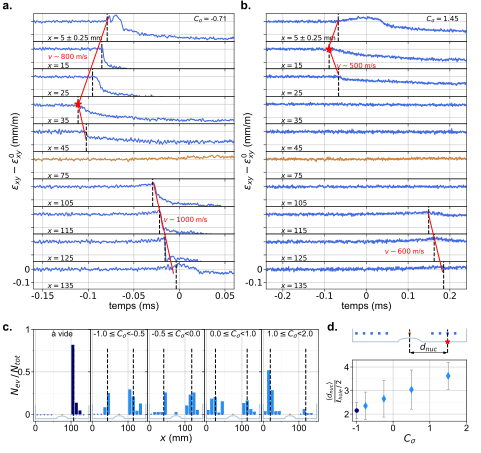
\includegraphics[scale=1]{../Figures_chap_article/figure_4.pdf}
\caption[Nucléation et propagation -- œil granulaire]{Évolution de la position du point de nucléation avec une augmentation de contraste de chargement. \textbf{a-b.}\,Mesure de $\Delta\varepsilon_{xy}(x,t)=\varepsilon_{xy}(x,t)-\varepsilon_{xy}^0(x)$ lors de la propagation d'une rupture rapide. Même code symbolique que Fig.\,\ref{fig:propagss}. \textbf{c.}\,Histogramme représentant la distribution des positions du point de nucléation pour les expériences à vide (bleu sombre) et les expériences granulaires (bleu clair), par plage de $C_\sigma$ (indiquées sur le graphe). Chaque barre correspond au nombre de ruptures s'étant initiées au niveau de la jauge associée $N_{ev}$, normalisé par le nombre total de ruptures $N_{tot}$ dans cette plage de $C_\sigma$. \textbf{d.}\,Haut : représentation de la définition de la distance de nucléation. Bas : Valeur moyenne de la distance de nucléation $\mean{d_{nuc}}$, normalisée par la demi-longueur de l'œil granulaire $\ell_{eye}/2$, avec $\ell_{eye}=\SI{30}{\milli\meter}$. La moyenne est effectuée sur tous les évènements appartenant aux expériences de la plage de $C_\sigma$ considérée, et les barres d'erreur correspondent aux écarts types.}
\label{fig:papier4}
\end{figure}


L'ajout d'un milieu granulaire dans l'œil modifie le point de nucléation des ruptures. Les deux cas présentés en exemple (Fig.\,\ref{fig:papier4}a-b) pour $C_\sigma=-0.71$ et $C_\sigma=1.45$ montrent deux points de nucléation éloignés du coin droit de l'œil, respectivement à $x_{nuc}=\SI{35}{\milli\meter}$ et $x_{nuc}=\SI{15}{\milli\meter}$. Les signaux observés sont également moins amples que dans les expériences à vide en raison des plus faibles valeurs de $\sigma_{xy}^0$ dues à la diminution du temps de chargement normal avec $C_\sigma$ (Éq.\,\ref{eq:freqss}, Sec.\,\ref{sec:modiffreq}).
Dans le deuxième exemple, certains points de mesure ne subissent pas de diminution de $\varepsilon_{xy}$. L'absence de rupture au niveau de ces jauges constitue une indication de la longueur du patch en glissement lent. Une étude statistique de la distribution du point de nucléation est nécessaire.

\newpage


\subsubsection{Détermination de la distance de nucléation}

En déterminant le point de nucléation de chaque évènement de rupture, nous établissons des histogrammes de la localisation de la nucléation pour différentes valeurs de $C_\sigma$ (Fig.\,\ref{fig:papier4}c). Pour les expériences à vide, la plupart des ruptures nucléent au même endroit, proche du coin droit de l'œil à vide. Pour les expériences granulaires, même à faible $C_\sigma$, la distribution des positions du point de nucléation est plus large, à commencer par l'apparition de ruptures des deux côtés de l'œil. De plus, lorsque $C_\sigma$ augmente, le point de nucléation tend à s'éloigner de l'œil granulaire vers les bords extérieurs des blocs. Afin de caractériser cet effet, nous définissons la distance de nucléation $d_{nuc}$ de chaque évènement comme la distance entre le centre de l'interface et le point de nucléation $x_{nuc}$ (Fig.\,\ref{fig:papier4}d), soit en pratique, avec $L$ la longueur de l'interface,

\begin{equation}
d_{nuc}=\abs{x_{nuc}-\frac{L}{2}}
\end{equation}



La distance moyenne de nucléation $\mean{d_{nuc}}$ par plage de $C_\sigma$ augmente avec $C_\sigma$ (Fig.\,\ref{fig:papier4}d). Sachant que le glissement d'un patch dans une interface solide n'a lieu que lorsque les microcontacts frictionnels sont déjà affaiblis, le patch glissant ne peut pas être le siège de la nucléation d'une rupture. Par conséquent, le fait que $\mean{d_{nuc}}$ augmente avec $C_\sigma$ indique que la longueur du patch glissant augmente elle aussi avec le contraste de chargement.


Ainsi nous observons que le patch glissant, centré sur l'œil granulaire, s'étend bien à une partie des portions solide-solide de l'interface. Cette extension, quantifiée par $\mean{d_{nuc}}$, augmente avec le contraste de chargement. Ce résultat est cohérent avec nos observations précédentes, et clarifie le mécanisme par lequel l'interface se déstabilise lorsque $C_\sigma$ augmente. Pour autant la faible résolution spatiale de nos mesures nous limite dans la détermination de la longueur du patch. À cet effet, nous étudions l'évolution lente du cisaillement au cours des périodes inter-évènement.




% Le patch glissant servirait alors de précurseur à la nucléation d'une rupture. Un précurseur est une rupture pré-existante, c'est à dire une ligne le long de laquelle les contraintes à l'interface ont déjà été partiellement relâchées. Ce précurseur se déstabilise et s'étend en une rupture complète de l'interface lorsque la contrainte cisaillante dépasse une valeur seuil, donnée par le critère de Griffith en mécanique de la fracture élastique. Ce scénario nécessite pour être valide que le patch glissant, incluant l'œil granulaire et une partie de l'interface solide-solide de part et d'autre de celui-ci, relâche les contraintes qui lui sont appliquées au cours de la phase inter-évènement. Notre méthode de suivi optique de l'interface a révélé un glissement, qui s'accompagne nécessairement d'un relâchement de contraintes (Fig.\,\ref{fig:papier3}), mais la faible résolution spatiale de nos mesures nous limite. Cependant, la mesure des évolutions lentes du tenseur des déformations tout au long des expériences nous permet de déterminer la longueur de ce patch.


\section[Extension du patch en glissement avec le contraste de chargement]{\fontsize{15}{12}\selectfont Extension du patch en glissement avec le contraste de chargement}
\label{sec:longueurpatch}



En suivant le glissement lent de l'interface pendant les périodes inter-évènement, nous avons mis en évidence l'existence d'un patch glissant. En déterminant la distance de nucléation moyenne des évènements de rupture associés au glissement rapide, nous avons montré que la portion d'interface dans laquelle ne nucléent pas de ruptures, que nous associons au patch glissant, n'est pas limitée au seul œil granulaire, et que sa longueur augmente avec $C_\sigma$. Nous allons maintenant mesurer l'extension de ce patch par une mesure directe, et en montrer l'adéquation avec la mesure par détermination des points de nucléation des ruptures.

\subsection{Principe de la mesure}
Pour un mouvement de stick-slip idéal, les phases de stick correspondent à une séquence de chargement élastique de l'interface. Le PMMA ayant, à basse fréquence de sollicitation, un module d'Young constant, l'augmentation des déformations et des contraintes est linéaire avec le déplacement imposé au bloc. Dans nos expériences, ce chargement est effectué à vitesse constante, nous nous attendons donc à une augmentation linéaire de $\varepsilon_{xy}(x,t)$ et $\sigma_{xy}(x,t)$ en fonction du temps en tout point de l'interface. Si en revanche une portion de l'interface est découplée ($\phi<1$) et donc en glissement lent, les contraintes qui lui sont appliquées sont partiellement relâchées pendant la phase de chargement. L'évolution de $\varepsilon_{xy}(x,t)$ en fonction du temps n'est alors plus linéaire, mais moindre, c'est-à-dire sous-linéaire. Grâce à l'acquisition lente (\SI{315}{\hertz}) des signaux des jauges de déformation tout au long de nos expériences, nous pouvons observer les séquences de chargement entre chaque évènement et pour chaque jauge (Fig.\,\ref{fig:papier5}). Ce faisant, nous pouvons déterminer si un chargement est linéaire ou sous-linéaire. Cette détermination est effectuée manuellement pour chaque évènement et chaque jauge. Une automatisation de cette détection par un ajustement linéaire en temps de $\varepsilon_{xy}(x_i,t)$ est une perspective d'amélioration de la mesure.



\subsection{Apparition de chargements sous-linéaires}


\begin{figure}[p]
\centering
\includegraphics[scale=1]{../Figures_chap_article/figure_5.pdf}
\caption[Chargements sous-linéaires et linéaires]{Évolution de la longueur du patch glissant avec le contraste de chargement. Le code couleur est le même que pour Fig.\,\ref{fig:papier4}. \textbf{a-b.}\,Évolution temporelle des déformations cisaillantes $\varepsilon_{xy}(x,t)$ à \SI{315}{\hertz} pour les 10 jauges de déformation, pour une expérience à vide (\textbf{a}) et une expérience granulaire à $C_\sigma=1.13$ (\textbf{b}). Pour chaque phase inter-évènement, chaque jauge est classée comme linéaire (L) ou sous-linéaire (SL). Les lignes noires en pointillés (\textbf{b}) sont un ajustement de $\varepsilon_{xy}$ sur les derniers instants avant un évènement rapide. \textbf{c.}\,Compte de la proportion de phases inter-évènement sous-linéaires par jauge $N_{SL}$, normalisé par le nombre total de ces phases $N_{ev}$, pour chaque plage de $C_{\sigma}$. \textbf{d.}\,Valeur moyenne de la longueur du patch glissant $\mean{\ell_{slip}}$, normalisée par la longueur de l'œil granulaire $\ell_{eye}=\SI{30}{\milli\meter}$.}
\label{fig:papier5}
\end{figure}


Pour une expérience à vide, comme attendu, quasiment toutes les jauges montrent une évolution linéaire de leur signal durant toutes leurs séquences de chargement (Fig.\,\ref{fig:papier5}c). L'interface à vide se comporte comme une interface solide-solide homogène. Pour les expériences granulaires, certaines jauges montrent un comportement sous-linéaire au cours d'une partie des séquences de chargement. L'augmentation du chargement cisaillant débute de manière linéaire tant que le couplage de l'interface est proche de $\phi=1$, puis s'incurve lorsque $\phi<1$ (Fig.\,\ref{fig:papier5}b).


Dans l'exemple présenté, le comportement de deux points de mesure est explicité par des annotations, SL pour un chargement sous-linéaire, et L pour un chargement linéaire.
Au sein d'une même expérience, une jauge peut avoir un comportement différent pour différents évènements, comme montré par la dernière jauge ($x=\SI{135}{\milli\meter}$) de la Figure\,\ref{fig:papier5}b.
Cette évolution indique que la longueur du patch glissant évolue au cours de l'expérience, et l'étude de sa dynamique pourrait faire l'objet d'un approfondissement.
Certaines jauges, comme la première ($x=\SI{5}{\milli\meter}$) de la figure\,\ref{fig:papier5}b, exhibent même un chargement plus rapide que linéaire. Ceci pourrait indiquer que la contrainte relâchée par le patch glissant s'accumule en ses coins.

À temps très court (moins de \SI{500}{\milli\second} après l'évènement) et même pour les jauges ayant dans l'ensemble une évolution linéaire, il est possible d'observer que le signal de $\varepsilon_{xy}$ augmente logarithmiquement. Cette augmentation  est due au vieillissement de l'interface à la fin d'une phase de glissement rapide, et est discutée dans le Chapitre\,\ref{sec:chapintro} (Sec.\,\ref{sec:aging}).

Pour chaque expérience et pour chaque jauge, nous mesurons la proportion des séquences de chargement exhibant un comportement sous-linéaire, $N_{SL}/N_{ev}$. Une grande valeur de cette fraction indique que l'interface au niveau de la position de la jauge concernée est peu couplée, fréquemment en glissement inter-évènement. Cette mesure est représentée sous la forme d'un histogramme en fonction des valeurs de $C_\sigma$ (Fig.\,\ref{fig:papier5}c). La distribution ainsi représentée s'élargit lorsque $C_\sigma$ augmente, indiquant que l'extension du patch glissant augmente avec le contraste de chargement.




\subsection{Mesure de l'extension du patch glissant}

\begin{figure}[h!]
\centering
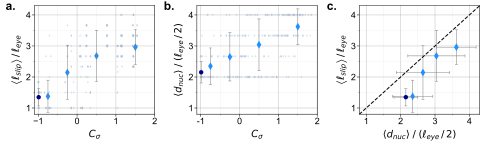
\includegraphics[scale=1]{../Figures_chap_article/ell_triple.pdf}
\caption[Évolution de $\ell_{slip}$ et $d_{nuc}$ en fonction de $C_\sigma$]{Évolution de la taille du patch glissant en fonction du contraste de chargement. \textbf{a.}\,Mesure de la longueur du patch obtenue avec la détermination du point de nucléation moyen des ruptures. \textbf{b.}\,Mesure de la longueur du patch obtenue avec l'identification des jauges sous-linéaires. Les points en gris clair correspondent chacun à un évènement. \textbf{c.}\,Comparaison des deux méthodes.}
\label{fig:ell_triple}
\end{figure}

L'extension spatiale de la distribution obtenue nous informe sur la longueur probable du patch glissant, pour une plage de $C_\sigma$ donnée. Afin de quantifier cette extension nous pouvons déterminer par évènement la longueur $\ell_{patch}$ du patch glissant. Nous la calculons comme la distance entre la première et la dernière position mesurées comme sous-linéaires.  Cette grandeur, moyennée par plage de $C_\sigma$, est bien une fonction croissante du contraste de chargement (Fig.\,\ref{fig:papier5}).
De plus ce résultat est cohérent avec la mesure de $\mean{d_{nuc}}$ effectuée précédemment, puisque les deux longueurs normalisées $\mean{\ell_{patch}}/\ell_{eye}$ et $\mean{d_{nuc}}/(\ell_{eye}/2)$ sont comparables, en particulier lorsque le patch n'est pas restreint à l'œil granulaire (Fig.\,\ref{fig:ell_triple}).


Nous avons donc montré que le patch glissant s'étend au-delà de l'œil granulaire, et est caractérisé par un chargement sous-linéaire des mesures des déformations. Nous avons déterminé sa longueur par deux méthodes différentes donnant des résultats cohérents. La mesure de cette longueur nous apprend que l'augmentation de $C_\sigma$ est responsable d'une augmentation de la longueur du patch en glissement. Le mécanisme sous-jacent est détaillé dans la section suivante.

\newpage

\section{Le patch en glissement joue le rôle d'un pré-crack}

L'ensemble de nos mesures, en particulier la mesure conjointe de $\mean{d_{nuc}}$ et de $\mean{\ell_{patch}}$, montre que l'introduction d'une hétérogénéité consistant en un matériau granulaire induit un glissement lent localisé durant les périodes inter-évènement du cycle de stick-slip. Lorsque le chargement porté par l'œil granulaire augmente, le patch glissant s'étend, passant de la taille de l'œil à presque toute la longueur de l'interface. Parallèlement à cela, la fréquence du stick-slip augmente, révélant que les initiations de ruptures deviennent plus fréquentes avec l'augmentation du chargement porté par le milieu granulaire (Fig.\,\ref{fig:loadingcontrast},\,\ref{fig:frequencyfn} et\,\ref{fig:papier3}b). Notre interprétation de ce comportement est que le patch glissant agit comme un précurseur de fracture, ou pré-crack, le long de l'interface.

Cette section détaille le mécanisme par lequel un pré-crack dans un milieu homogène se déstabilise et se propage en rupture dynamique. Nous y montrons le parallèle entre ce mécanisme et le système d'interface à œil granulaire, et présentons les limites de notre étude dans la caractérisation quantitative de ce parallèle.



\subsection{Qu'est-ce qu'un pré-crack ?}


\begin{figure}[h]
\centering
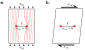
\includegraphics[scale=1]{../Figures_chap_article/crack_griffith.pdf}
\caption[Accumulation des contraintes en pointe de fissure]{Représentation schématique de deux pré-cracks. \textbf{a.}\,Pré-crack en mode\:\textsc{i} ou mode d'extension. Une contrainte d'étirement $\sigma_{yy}$ homogène est appliquée au système. Les lignes rouges représentent les lignes de force dans le matériau. Une concentration des lignes de force indique une augmentation de la contrainte locale\,\cite{ohring_engineering_1995}. \textbf{b.}\,Pré-crack de longueur $\ell$ en mode\:\textsc{ii} ou mode de cisaillement. Une contrainte de cisaillement $\sigma_{xy}$ homogène est appliquée au système. Les cercles rouges indiquent une concentration des contraintes.}
\label{fig:griffith}
\end{figure}


Lorsqu'une contrainte $\sigma$ est appliquée aux bords d'un matériau élastique isotrope, elle est transmise à l'intérieur de celui-ci selon la loi de Hooke. Si le milieu est homogène, chaque volume infinitésimal du matériau supporte la même contrainte, mais si un défaut apparaît, il est le siège d'une concentration de contrainte, ce qui en fait un point de faiblesse du matériau. Un pré-crack est un défaut du matériau consistant en une surface le long de laquelle les contraintes sont nulles.

Un exemple de pré-crack dans un matériau soumis à une contrainte d'extension (dite de mode\:\textsc{i}) est une déchirure dans une feuille fine que l'on étire (Fig.\,\ref{fig:griffith}a). Lors de l'étirement de la feuille, la longueur de la déchirure ne supporte aucune contrainte $\sigma_{yy}$. Sa pointe en revanche accumule de plus grandes contraintes que le reste du matériau, ce qui mène à terme à sa propagation, et à la déchirure complète de la feuille. Le cas d'un mode de cisaillement (mode\:\textsc{ii}) est similaire, la contrainte nulle le long du pré-crack étant la contrainte cisaillante $\sigma_{xy}$ (Fig.\,\ref{fig:griffith}b). Pour une interface frictionnelle, la situation est analogue, à ceci près que le pré-crack que constitue un patch glissant à l'interface entre deux blocs ne relâche pas l'entièreté des contraintes qui lui sont appliquées, puisqu'il est dans un régime de frottements dynamiques. La contrainte qu'il porte est alors la contrainte résiduelle $\sigma_r$ (introduite Sec.\,\ref{sec:nuccontexte}).

\pagebreak

Notre hypothèse est que le patch glissant agit comme un pré-crack en mode de cisaillement pour l'interface en œil granulaire.


\subsection{Critère de Griffith pour l'initiation d'une fracture}
\label{sec:griffith}


\subsubsection{Expression du critère}

Lorsque la contrainte appliquée à l'interface est suffisante, le pré-crack se déstabilise en rupture dynamique et se propage. Le critère d'initiation ce cette propagation, nommé \textit{critère de Griffith}, est que le taux de restitution d'énergie $G$, correspondant à l'énergie perdue par le relâchement des contraintes le long d'une fracture, est égal à l'énergie de fracture du matériau $\Gamma$, correspondant à l'énergie nécessaire à la création d'une unité de surface libre en son sein\,\cite{griffith_phenomena_1921,freund_dynamic_1990} (Sec.\,\ref{sec:LEFM}). Dans le cas d'un solide infini sous chargement homogène en mode\:\textsc{i}, ce critère mène à une expression de la contrainte macroscopique limite $\sigma_c$ pour laquelle une fissure de longueur $\ell$ donnée se déstabilise.

\begin{equation}
\sigma_c=\sqrt{\dfrac{\Gamma E}{(1-\nu^2)\ell}}
\end{equation}


Ainsi la contrainte nécessaire pour déstabiliser un pré-crack est une grandeur décroissante de la longueur de celui-ci. Dans le cas d'une interface frictionnelle, une fissure ne relâche que partiellement les contraintes à $\sigma_r$\,\cite{svetlizky_classical_2014}. Étant donné que dans nos expériences le patch glissant est une ligne de relâchement des contraintes cisaillantes, il est raisonnable de penser qu'un critère similaire à celui de Griffith puisse s'appliquer, l'équation $G=\Gamma$ permettant alors de relier $\sigma_c-\sigma_r$ à $\ell$.



%le critère devient
%\begin{equation}
%\Delta\sigma_{xy} = \sigma_c-\sigma_r=\sqrt{\dfrac{\Gamma E}{(1-\nu^2)\ell}}
%\label{eq:griffith}
%\end{equation}



\subsubsection{Limites de notre dispositif}


Afin de valider l'hypothèse selon laquelle le patch glissant agit comme un pré-crack en mode de cisaillement, il serait a priori possible de comparer nos résultats aux prédictions du modèle de pré-crack de Griffith, notamment par une évaluation de $\Gamma$ par la mesure de $\sigma_{xy}^0-\sigma_r$ au point de nucléation de la rupture. Cependant notre dispositif expérimental, ainsi que la nature de l'interface en œil granulaire, ne nous le permettent pas. En effet nous avons accès aux valeurs de ${\sigma_{xy}^0-\sigma_{xy}^{\infty}}$, où $\sigma_{xy}^{\infty}$ correspond à la contrainte après le relâchement inertiel des contraintes par le glissement de l'interface,
%ainsi qu'à $\Delta F_S$,
mais nous n'avons pas accès à $\sigma_{r}$\,\cite{svetlizky_classical_2014}.
De plus, la dépendance spatiale du chargement cisaillant due à l'hétérogénéité de composition, ainsi que le gradient de contrainte normale dû au contraste de chargement (Fig.\,\ref{fig:loadingcontrast}), complexifient d'autant plus l'estimation quantitative de $G$, qui nécessite une mesure de $\sigma_{xy}^0$ d'une résolution spatiale que notre dispositif expérimental ne nous permet pas d'atteindre.


La valeur locale de l'énergie de fracture $\Gamma$ affecte également $\sigma_c$. L'énergie de fracture dépend linéairement de la contrainte normale locale\,\cite{bayart_fracture_2016,bayart_slippery_2016}, et en raison de la distribution très hétérogène de cette contrainte le long de notre interface, nous ne pouvons pas la déterminer précisément, mais seulement obtenir des informations indirectement. Cependant, le critère de Griffith doit être localement satisfait au point d'initiation de la rupture pour que celle-ci se propage. Ainsi une mesure de la contrainte normale au point de nucléation nous donne une indication de la variation de l'énergie de fracture avec le contraste de chargement. La Figure\,\ref{fig:papier6}c montre l'évolution de la valeur moyenne de $\sigma_{yy}$ au point de nucléation juste avant l'évènement de glissement rapide, $\mean{\sigma_{yy}^0(x_{nuc})}$, en fonction de $C_\sigma$. Ce graphique montre une tendance décroissante, ainsi la variation de l'énergie de fracture $\Gamma $ au point de nucléation pourrait jouer un rôle dans la réduction de la contrainte critique $\sigma_c$ de déstabilisation de la rupture. Cet effet s'ajoute à celui de l'allongement du patch glissant, et les deux effets ne peuvent pas être contrôlés de manière indépendante. Cependant nous pouvons vérifier que le comportement du système en présence d'un patch glissant suit les mêmes tendances qu'en présence d'un pré-crack classique.





\subsection{Mécanisme complet de déstabilisation de l'interface}


En conclusion, l'œil granulaire créé un patch en glissement, qui agit comme un pré-crack réduisant $\sigma_c$, et provoquant une déstabilisation précoce de l'interface par rapport à une situation sans grains.

\vspace{1cm}

\begin{figure}[htb]
\centering
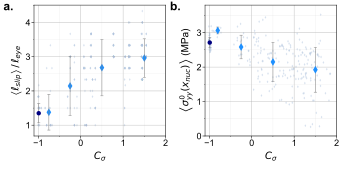
\includegraphics[scale=1]{../Figures_chap_article/figure_6.pdf}
\caption[Déstabilisation de la rupture]{Longueur du patch glissant et contrainte normale menant à la déstabilisation de la rupture. \textbf{a.}\,Évolution de la longueur du patch glissant normalisée $\mean{\ell_{patch}}/\ell_{eye}$ (Fig.\,\ref{fig:papier5}c) en fonction de $C_\sigma$, pour les expériences à vide (cercle bleu sombre) et les expériences granulaires (diamants en bleu clair). Les barres d'erreur correspondent aux écarts types des distributions présentées en gris. Figure identique à Fig.\,\ref{fig:ell_triple}a. \textbf{b.}\,Valeurs moyennes de $\sigma_{yy}^0(x_{nuc})$, la contrainte normale mesurée au point de nucléation $x_{nuc}$ pour chaque évènement de glissement rapide, pour chaque plage de $C_\sigma$ considérée. Les mesures de $\sigma_{yy}^0(x_{nuc})$ pour chaque évènement sont représentées en gris.}
\label{fig:papier6}
\end{figure}



\newpage

L'insertion d'une hétérogénéité de composition à l'interface sous forme d'un œil granulaire entraîne la formation d'un patch en glissement lent entre les évènements de rupture rapide. Ce patch en glissement lent n'est pas limité à l'œil granulaire, et s'étend au sein des portions solide-solide de l'interface, comme montré par la mesure de $x_{nuc}$ (Fig.\,\ref{fig:papier4}). Une augmentation du chargement porté par le milieu granulaire, donc de $C_\sigma$, entraîne une augmentation de la taille de ce patch, estimée par $\ell_{patch}$ (Fig.\,\ref{fig:papier6}).  Le patch en glissement lent agit comme un pré-crack, dans lequel les contraintes sont partiellement relâchées. Selon le critère de Griffith, plus la longueur $\ell_{patch}$ est grande, plus le chargement cisaillant $\Delta\sigma = \sigma_c-\sigma_r$ nécessaire pour le déstabiliser en rupture dynamique est faible (Sec.\,\ref{sec:griffith}). L'augmentation de $C_\sigma$ entraîne également un deuxième effet, qui est la réduction de l'énergie de fracture $\Gamma $ au point de nucléation (Fig.\,\ref{fig:papier6}). L'effet de la diminution de $\Gamma $ se cumule à celui de l'augmentation de $\ell_{patch}$. Le patch en se déstabilisant donne naissance à une rupture dynamique se propageant à l'interface. Plus l'écart de contrainte $\Delta\sigma$ est faible, moins le temps de chargement à vitesse constante nécessaire pour l'atteindre est faible, et donc plus $\mean{\Delta T}$ est faible (Éq.\,\ref{eq:freqss}).


Ce mécanisme d'extension d'un précurseur de fissure conduisant à une augmentation de la fréquence de stick-slip, ainsi qu'à une diminution locale de l'énergie de rupture, n'est pas trivial. Un scénario évident serait que le glissement lent de l'œil granulaire induit une concentration de contraintes à la jonction entre la zone découplée, c'est à dire l'œil, et la zone partiellement couplée, c'est à dire les sections solide-solide. Dans ce scénario, la surcharge aux coins du patch entraînerait la propagation dynamique de la rupture en atteignant la résistance au cisaillement des contacts, comme cela a été observé dans différents systèmes\,\cite{bedford_fault_2022,gvirtzman_nucleation_2021}. Cependant, ce n'est pas ce que nous observons. Le glissement lent à l'intérieur du patch granulaire induit un glissement lent des contacts voisins plutôt qu'une rupture dynamique. Ainsi, la zone de glissement lent affecte la dynamique de rupture tout le long de l'interface en modifiant la nucléation de la rupture, plutôt qu'en agissant localement sur la distribution des contraintes. Ce résultat contraste avec d'autres études dans lesquelles les propriétés de frottement des hétérogénéités interfaciales évoluent avec l'histoire du glissement\,\cite{cebry_creep_2022,bedford_fault_2022,rubino_intermittent_2022}, ou dans lesquelles une fréquence accrue de stick-slip s'explique par la propagation de ruptures arrêtées par les hétérogénéités, qui agissent comme une barrière\,\cite{bayart_rupture_2018,buijze_effects_2021,ma_period_2001}. 




\section{Discussion}

Nous avons observé un mécanisme permettant à un patch glissant de déstabiliser une interface frictionnelle. Le patch, créé par l'insertion d'un milieu granulaire à l'interface, s'étend au-delà de l'œil dans lequel ce dernier est encapsulé. Quelle est le mécanisme derrière cette extension ?

\subsection{Mécanismes du glissement lent}

Pourquoi certaines portions d'interfaces glissent lentement alors que d'autres se rompent lors d'évènements rapides ? Deux mécanismes peuvent être invoqués pour répondre à cette question. Le premier mécanisme est celui du glissement lent des microcontacts, surchargés par l'œil granulaire, à des vitesses de l'ordre de quelques micromètres par seconde (Fig.\,\ref{fig:papier2}d). Ce régime de glissement lent a été observé pour différents systèmes expérimentaux\,\cite{heslot_creep_1994,rabinowicz_intrinsic_1958}. Les phénomènes de vieillissement des contacts (Sec.\,\ref{sec:aging}), renforçant l'interface, agissent de concours avec les phénomènes de déformation plastique induits par le chargement cisaillant lent de l'interface. Les échelles de temps des deux phénomènes sont comparables, et peuvent mener à un glissement lent plutôt qu'à une fracture dynamique. Le second mécanisme est la dilatance du milieu granulaire induite par son cisaillement. Un matériau granulaire se dilate lorsqu'il est cisaillé, ce qui peut relâcher localement la contrainte normale portée par les portions solides d'interface à proximité, et mener à un glissement stable\,\cite{svetlizky_classical_2014}. Dans nos expériences, nous observons une réduction locale des contraintes aux bords de l'œil granulaire lorsque le chargement porté par celui-ci augmente, mais pas d'annulation (Fig.\,\ref{fig:loadingcontrast}). Cette réduction locale de la contrainte normale pourrait expliquer la transition de stick-slip à glissement stable\,\cite{baumberger_crossover_1994,leeman_laboratory_2016}. Ce second mécanisme met en avant l'importance de la prise en compte du comportement mécanique des hétérogénéités dans les modèles théoriques et numériques.


\subsection{Implications en mécanique des failles}


L'influence des portions de failles asismiques et des séismes lents sur le comportement des portions sismiques bloquées est un sujet de recherche actif, et est encore mal comprise \cite{bedford_fault_2022, lindsey_slip_2021, tan_connecting_2020, leeman_frictional_2018, burgmann_geophysics_2018, radiguet_triggering_2016}. Nos expériences permettent d'explorer la dynamique complexe de ces failles en contrôlant les ingrédients responsables de leur complexité. Nos observations peuvent par exemple correspondre à un scénario où un glissement lent induit des micro-séismes répétés\,\cite{tan_connecting_2020} plutôt qu'une occurrence d'un évènement de magnitude élevée\,\cite{ong_factors_2021, kircher_when_2006}. Dans notre étude, l'amplitude de l'évènement, c'est-à-dire la chute de force, est contrôlée par la longueur du patch glissant plutôt que par la quantité de glissement lent. Cette étude soulève également la question des zones de failles à surveiller. Si la zone de glissement lent peut s'étendre le long d'une faille, comme le suggèrent nos résultats, il est important de surveiller l'évolution de cette zone pendant les phases intersismiques.



\subsection{Perspectives}


Notre étude met en évidence un mécanisme d'interaction entre une zone découplée, en glissement lent, et une zone couplée, verrouillée. Les frontières de la zone en glissement ne sont pas limitées à l'hétérogénéité de composition que constitue l'œil granulaire, mais s'étendent dans les portions solide-solide de l'interface. Le glissement lent que nous observons pourrait être une manifestation d'un front de nucléation, comme observé expérimentalement\,\cite{cebry_creep_2022,gvirtzman_nucleation_2021,latour_characterization_2013} et dans des modèles\,\cite{brener_unstable_2018,de_geus_how_2019} dans des études précédentes. La résolution temporelle de notre dispositif n'est cependant pas suffisante pour caractériser la dynamique de décrochage des contacts. Cette question, particulièrement pertinente dans la prévention des risques sismiques\,\cite{rolandone_seismic_2022,lindsey_slip_2021}, est laissée pour des études futures, qui devront élucider le mécanisme derrière l'extension de la zone de glissement lent. De plus, une estimation quantitative de $\Gamma$ et $G$ nous doterait d'un critère pour la propagation de la rupture, fournissant des informations sur la longueur de déstabilisation de la zone de glissement, pour des conditions de chargement connues. Cette mesure nous donnerait un pouvoir prédictif sur le comportement de l'interface. La modélisation de l'extension d'une zone de glissement lent peut fournir des résultats intéressants à cette fin.
%Enfin, des mesures acoustiques expérimentales permettraient de relier le contenu des ondes sismiques aux propriétés de leur source, qui sont inaccessibles dans les failles naturelles.



\section{Conclusion}

Au cours de ce chapitre, nous avons étudié l'influence d'une hétérogénéité de composition au sein d'une interface frictionnelle. Cette interface est formée par deux blocs de PMMA mis en contact par une presse et cisaillés. Nous avons montré dans une première partie que l'inclusion d'une hétérogénéité sous la forme d'un œil contenant un milieu granulaire perturbe le mouvement de stick-slip de l'interface. Plus le milieu granulaire est dense, plus la période du stick est courte. Nous avons ensuite mis en évidence, grâce à des mesures optiques des déplacements à l'interface, l'existence d'un patch en glissement lent à l'interface, glissant d'autant plus que la densité du milieu granulaire, quantifiée par le contraste de chargement $C_\sigma$, augmente. Ce patch est centré sur l'œil granulaire mais ne se limite pas à celui-ci. En effet nous avons montré grâce aux mesures conjointes du tenseur des déformations à basse fréquence tout au long des expériences et par salves à haute fréquence lors des évènements rapides que lorsque $C_\sigma$ augmente, le patch s'étend dans les portions solide-solide de l'interface. Ce patch agit comme un crack de Griffith en mode\:\textsc{ii}, dont la longueur augmente avec $C_\sigma$, déstabilisant l'interface.


En résumé, nous avons montré qu'une zone en glissement lent au sein d'une interface frictionnelle agit comme un précurseur de rupture, qui induit une déstabilisation précoce de l'interface entière en abaissant le niveau de contrainte auquel la fissure se propage, suivant la même tendance qu'un critère de Griffith dérivé de la mécanique de la rupture. Ce mécanisme entraîne une modification du cycle de stick-slip. Notre étude met en évidence une description basée sur la mécanique de la rupture de l'effet d'une hétérogénéité sur la dynamique de l'interface frictionnelle. Elle offre ainsi de nouvelles perspectives pour rendre compte de la complexité des failles dans les modèles et pour faire progresser la compréhension de la diversité du comportement des failles sismiques.









